\documentclass{article}
\usepackage[a4paper, total={6.5in, 10in}]{geometry}
\setlength{\parindent}{0pt}
\usepackage{tcolorbox}
\tcbset{colback=white!94!black, colframe=black!60!white, coltitle = white, boxrule=0.8pt, arc=2mm}
\newtcolorbox{boxs}[2][]{title= #2,#1}
\usepackage{datetime2}
\usepackage[british]{babel}
\usepackage{amsfonts}
\usepackage{amsmath}
\usepackage{pgfplots}
\pgfplotsset{compat=1.18}


\title{\textbf{Advanced Calculus HW 2}}
\author{Robert O'Connell}
\date{\today}
\begin{document}
\maketitle
\vspace{5mm}

\subsection*{Question 1}

\subsubsection*{(a)}
To find \(\mathcal{D}(\vec{r})\) we need to find the intersections of the natural domains of the component
functions.
\[
\ln(t), \quad -t, \quad t^2
\]
\[
t>0, \quad t \in \mathbb{R}, \quad t \in \mathbb{R}
\]
\[
t > 0
\]
\(\mathcal{D}(\vec{r}) = t, \quad t > 0\)

\subsubsection*{(b)}
\[
\frac{d\vec{r}}{dt} = \frac{1}{t} \hat{i} -1 \hat{j} + \frac{t}{2} \hat{k}, \quad t > 0
\]
Yes, this curve is smoothly parameterized since \(\vec{r}(t) \neq 0 \quad \forall \ t > 0\) since \(-1 \neq 0\) and all component functions 
are continuous for \(t >0\)

\subsubsection*{(c)}
\begin{align*}
    \left|\frac{d\vec{r}}{dt}\right| &= \sqrt{\left(\frac{1}{t}\right)^2 + (-1)^2  + \left(\frac{t}{2}\right)^2} \\
    &= \sqrt{\left(\frac{1}{4t^2}\right)(t^4 + 4t^2 + 4)} \\
    &= \left(\frac{1}{2t}\right)(t^2 + 2)
\end{align*}

\subsubsection*{(d)}
\begin{align*}
    \vec{T}(t) &= \frac{\vec{r} \ '(t)}{|\vec{r} \ '(t)|} \\
    &= \left(\frac{2t}{t^2 + 2}\right)\left(\frac{1}{t} \hat{i} -1 \hat{j} + \frac{t}{2} \hat{k}\right) \\
    &= \frac{2}{t^2 + 2} \hat{i} -\frac{2t}{t^2 + 2} \hat{j} + \frac{t^2}{t^2 + 2} \hat{k}, \quad t>0
\end{align*}


\subsubsection*{(e)}
\(\ln(t) = 0\) if and only if \(t = 1\)

\[
\vec{T}(1) = \frac{2}{3} \hat{i} - \frac{2}{3} \hat{j} + \frac{1}{3} \hat{k}
\]

The line, \(L\) is then
\[
L(\lambda) = \left(0, -1 , \frac{1}{4}\right) + \lambda\left(\frac{2}{3}, -\frac{2}{3}, \frac{1}{3}\right), \quad \lambda \in \mathbb{R}
\]


\subsection*{Question 2}
\subsubsection*{(a)}
To obtain the arc length parameterization of a generic smoothly parameterized vector valued function \(\vec{r}(t)\), 
first one computes the arc length as a function of \(t\) starting from a chosen reference point, say \(t_0\), by the 
formula 
\[
\vec{s}(t) = \int_{t_0}^{t} |\vec{r} \ ' (t')|dt'
\]
This gives \(s\), the arc length, as a function of \(t\), which you then solve for \(t\) in terms of \(s\), and plug 
these new values for \(t\) in terms of \(s\) back into \(\vec{r}(t)\) to get \(\vec{r}(s)\)


\subsubsection*{(b)}
\begin{align*}
    \vec{s}(t) &= \int_{5}^{t} \left(\frac{t'^2 + 2}{2t'}\right) dt' \\
    &= \int_{5}^{t} \left(\frac{t'}{2} + \frac{1}{t'}\right) dt' \\
    &= \left[\frac{t'^2}{4} + \ln(t')\right]_5^t \\
    &= \frac{t^2}{4} + \ln(t) - \frac{25}{4} - \ln(5)
\end{align*}

\begin{center}
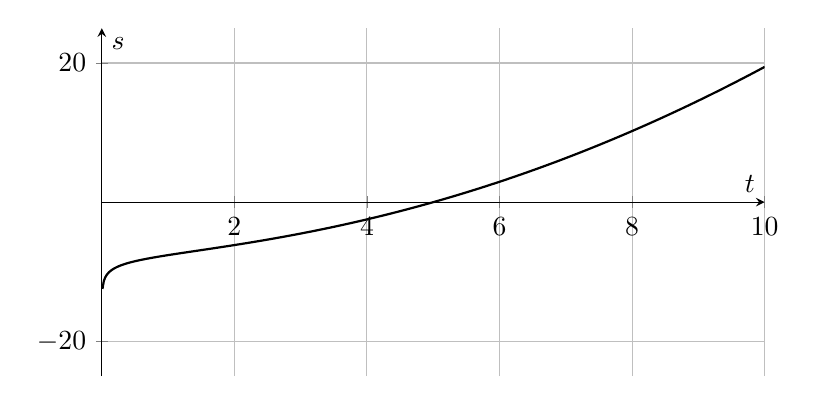
\begin{tikzpicture}
\begin{axis}[
    axis lines = middle,
    xlabel = $t$,
    ylabel = $s$,
    grid = both,
    width=10cm,
    height=6cm,
    xmin=0, xmax=10,
    ymin=-25, ymax=25
]
\addplot [domain=0.01:10, samples=500, black, thick] {(x^2)/4 + ln(x) - 25/4 - ln(5)};
\end{axis}
\end{tikzpicture}
\end{center}


\subsubsection*{(c)}
For the change of parameters to be smooth we need \(\frac{dt}{ds} \neq 0\) and \(\frac{dt}{ds}\) to 
be continuous.

We have
\[
s = \frac{t^2}{4} + \ln(t) - \frac{25}{4} - \ln(5)
\]
Then
\[
\frac{ds}{dt} = \frac{t}{2} + \frac{1}{t}
\]

\(\frac{ds}{dt}\) is continuous and \(\neq 0\), thus \(s(t)\) is strictly monotonic and \(\gamma^{-1}(t)\) is bijective, 
which implies \(\frac{dt}{ds} \neq 0\) and \(\frac{dt}{ds}\) continuous. 

Thus \(t = \gamma(s)\) is a smooth change of parameters
\end{document}